\documentclass[a4paper]{article}

%-----------------------------------------------------
\usepackage[a4paper, total={7in, 9in}]{geometry}
\usepackage{amsmath}
\usepackage{booktabs}
\usepackage{caption}
\usepackage{enumitem}
\usepackage{graphicx}
\usepackage{float}
\usepackage{inconsolata}
\usepackage{listings}
\usepackage{pstricks-add}
\usepackage{siunitx}
\usepackage[most]{tcolorbox}
\usepackage{tikz}
\usepackage{xfrac}
\usepackage{color}
\usepackage{multirow}
\usepackage{rotating}
\usepackage{url}

\usetikzlibrary{arrows}

%-----------------------------------------------------
\graphicspath{{./fig/}}
\setlength{\parindent}{0in}
%-----------------------------------------------------
\begin{document}
\title{ENG405 (Integrated Design Project): Statement of Work}
\author{Tatyana Maltseva (\textbf{s257346}), Sakon Nadthayai (\textbf{s245002}),\\ and Shane Reynolds (\textbf{s262538})}
\maketitle

\tableofcontents

\newpage

%-----------------------------------------------------
\section{Introduction}
As part of engineering degree at Charles Darwin University students require to undertake integrated design group project. An integrated group design project requires students to work together to complete the design task set by a client. The design project must meet client’s specification and performance criteria; it must be completed within the time frame; and satisfy all of the required milestones.\\

For electrical engineering students the design task is to build an autonomous robotic vehicle. The realisation of the project involves making a mathematical model, system simulation, designing control loops, completing the design of the vehicle mechanically and electrically and implementing the designed system using National Instruments MyRio hardware and LabVIEW software. 
%------------------------------------------------------
\section{Requirements \& Scope}
The main requirement of this project is to design and build an autonomous robotic vehicle that will traverse an enclosed area, which consists of obstacles. The robot will start from a randomised location, and needs to navigate to a designated finish position, in the shortest possible time. The finish location will be highlighted by a red marker, and once the robot has reached its objective, it must stop and provide a signal, physical or otherwise. These requirements can be found in more detail in the requirements matrix shown in Table 1.\\

\begin{table}[h]
\centering
\caption{Requirements matrix for the autonomous navigation robot}
\small
\begin{tabular}{cp{5.5cm}cp{5.5cm}}
\toprule
\textbf{Requirement} & \multirow{2}{*}{\textbf{Description}} & \textbf{Requirement} & \multirow{2}{*}{\textbf{Description}}\\
\textbf{Number} & & \textbf{Number} & \\
\midrule
R1 & The robot must act autonomously & R6 & The robot  needs to stop on top of the finish zone or within 100mm from the zone\\
 & & & \\
R2 & The robot is designed to act in a 3m $\times$ 6m environment & R7 & The robot must stop when it has reached the exit zone\\
 & & & \\
R3 & The robot can avoid obstacles of minimum size 55mm $\times$ 210mm $\times$ 297mm & R8 & The robot must signal once it has reached the exit zone\\
 & & & \\
R4 & The robot can identify and navigate to an exit zone, demarcated by a red square of size 420mm $\times$ 297mm & R9 & The robot chassis must use a Pololu Dagu Rover 5, two motor, tracked chassis with encoders (see Figure 1)\\
& & &\\
R5 & The robot must move from start to finish within 3 minutes & R10 & The robot must use an NI myRio 1900 powered by the Xilinx ZYNQ 7Z2010 (see Figure 2), or an Arduino powered by the ATmega328 for the embedded system.\\
\bottomrule
\end{tabular}
\end{table}

The scope of the project works include the following items:
\begin{itemize}
\item Statement of work
\item Critical analysis of options
\item Demonstration \& presentation which consists of:
\begin{itemize}
\item Initial demonstration of obstacle avoidance, final demonstration of full system functionality, and a 10 minute presentation outlining design process, and showcasing final system.
\end{itemize}
\end{itemize}

\begin{figure}[h]
\centering
\begin{minipage}{0.45\textwidth}
\centering
\frame{\includegraphics[height=5cm]{robot_image}}
\caption{Pololu Dagu Rover 5, two motor, tracked chassis with encoders}
\end{minipage}
\hspace{1cm}
\begin{minipage}{0.45\textwidth}
\centering
\frame{\includegraphics[height=5cm]{my_rio_image}}
\caption{NI myRio powered by the Xilinx ZYNQ 7Z2010 microprocessor}
\end{minipage}
\end{figure}

%------------------------------------------------------
\section{Design Options}
There are a number of competing designs which would serve the project's intended objectives, and still fall within the purview of the scope. Broadly, in terms of complexity, these solutions can be placed into one of three categories: low, moderate, or high. Typically, the higher the complexity the greater the cost of the project, however, with increased complexity there is an expectation of greater performance and efficiency. This section of the report provides a high level overview for each of the three options, making elementary design recommendations for each. The section concludes by nominating a preferred solution, and proposing future lines of enquiry which need to be directed to the client.

\subsection{Low Design Complexity}
One of the simplest and lowest cost designs, would be the implementation of a finite state machine. The robot chassis would be equipped with four sensors: one IR sensor on the front to check for an obstacle free path forward, and two on the sides of the robot to provide assurance the robot will not collide with walls to the left and right. A final sensor could be employed on rear of the robot chassis, pointing towards the floor, which would be used to detect if the robot is currently placed on the red exit panel. Kumar et alias (2016) suggest two types of IR sensor for this implementation: a SHARP GP2D120 (4cm to 30cm range) for the sides of the robot, and a SHARP GP2Y0A21YK0F (10cm to 80cm range) for the front of the robot. A very simple example of what the robot’s operation might look like can be seen in Figure 3 - this robot has 4 states of operation in which it can operate:
\begin{enumerate}
\item \textbf{Forward:} the robot operates in this mode of operation provided there are no obstacles present in the robot’s path (within some certain distance threshold). The robot will maintain a constant forward velocity in this mode - perhaps implemented with PID control. If the robot’s sensor detects an obstacle in the path, then the robot would transition to the stop state. Finally, if the robot detects that it is on the red ‘exit’ panel, then the robot would move to the finish state.
\item \textbf{Stop:} in the stop state the robot would set the velocity to zero, and checking the encoder that this was true. This state would persist if the robot was not stopped. If the robot was stopped, and the path was blocked, then the robot would transition to the turn state. If the robot was stopped, and the path was not blocked, then the robot would transition back to the forward state.
\item \textbf{Turn:} in the turn state, the robot would move the left motor forward, and the right motor in reverse, to perform a 90 degree pivot turn (a turn on the spot). Once the robot has complete the 90 degree turn, the robot will automatically transition state back to the stop state.
\item \textbf{Finish:} if the robot transitions to this state, then the robot is current located over the red exit panel for the environment. The robot will signal (audio or otherwise) that it is exiting the environment. The robot cannot transition out of this state - it is persistent.
\end{enumerate}

\newpage

\begin{figure}[h]
\centering
\begin{minipage}{0.45\textwidth}
\centering
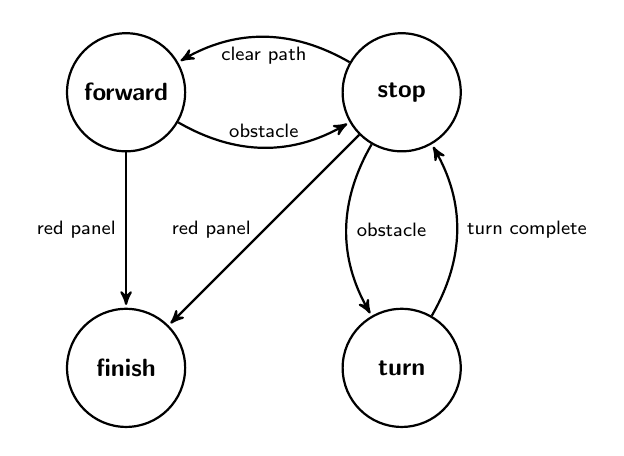
\begin{tikzpicture}[->,>=stealth',shorten >=1pt,auto,node distance=3.5cm,
                    thick,main node/.style={circle,minimum size=1.5cm,draw,font=\sffamily\small\bfseries}]
% Create nodes for the graph
\node[main node] (forward) {forward};
\node[main node] (stop) [right of=forward] {stop};
\node[main node] (turn) [below of=stop] {turn};
\node[main node] (finish) [below of=forward] {finish};

% Create edges for the graph
\path[every node/.style={font=\sffamily\scriptsize}]
(forward) edge [bend right] node [above] {obstacle} (stop)
(stop) edge [bend right] node [below] {clear path} (forward)
(forward) edge node [left] {red panel} (finish)
(stop) edge node [xshift=-1.3cm,yshift=0.25cm] {red panel} (finish)
(stop) edge [bend right] node [right] {obstacle} (turn)
(turn) edge [bend right] node [right] {turn complete} (stop);
\end{tikzpicture}
\caption{A state transition diagram which helps to explain how the robot moves from state to state in operation.}
\end{minipage}
\hspace{1cm}
\begin{minipage}{0.45\textwidth}
\centering
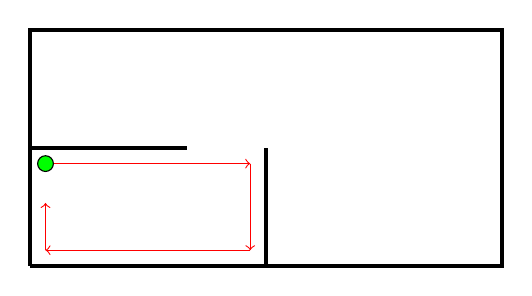
\begin{tikzpicture}
% Drawing environment
\draw[thick, line width=1.5pt] (0,0)--(6,0)--(6,3)--(0,3)--(0,0);
\draw[thick, line width=1.5pt] (3,0)--(3,1.5);
\draw[thick, line width=1.5pt] (0,1.5)--(2,1.5);

% Drawing robot path
\draw[red, ->] (0.2,1.3) -- (2.8,1.3);
\draw[red, ->] (2.8,1.3) -- (2.8,0.2);
\draw[red, ->] (2.8,0.2) -- (0.2,0.2);
\draw[red, ->] (0.2,0.2) -- (0.2,0.8);

% Drawing robot
\draw[fill=green] (0.2,1.3) circle (0.1cm);
\end{tikzpicture}
\caption{A simple example of environment design which would cause a basic robot, like the one detailed above, to fail. This figure shows the robot (a green circle) becoming trapped in an environment structure forever.}
\end{minipage}
\end{figure}

Whilst simple to implement, this design poses high risk of failure, and would need careful consideration of scenarios which may cause this failure. One elementary example of how this system might fail can be seen in Figure 4. Significant modifications to the scheme, and subsequent simulation or experimentation would need to be undertaken to ensure the required outcomes are met if this design is selected. A full description of the design option advantages, disadvantages, and hardware requirements can be found in Table XXXX.

\vspace{1cm}

\begin{table}[h]
\centering
\caption{Advantages, disadvantages and the hardware requirements for the design option}
\small\begin{tabular}{p{8cm}p{8cm}}
\toprule
\textbf{Advantages} & \textbf{Disadvantages}\\
\midrule
\begin{itemize}\item Simple to implement basic function \item Low cost \item Easy to source hardware \item Hardware has very few points of failure\end{itemize}
&
\begin{itemize}\item Environment topologies may exist that causes the robot to fail, or get trapped - these cases would need to be provided for individually \item The design may be too simple to navigate more complex environments completely\end{itemize}\\
\midrule
\textbf{Hardware Requirements} & \\
\midrule
\begin{itemize}\item Rover 5 chassis \item NI MyRio Xilinx 7Z2010 processor \item 4 Channel motor control unit \end{itemize} & \begin{itemize} \item 3 $\times$ SHARP GP2D120 \item 1 $\times$ SHARP GP2Y0A21YK0F\end{itemize}\\
\bottomrule
\end{tabular}
\end{table}

\begin{center}
\includegraphics[scale=0.1]{sensor_1_2}
\captionof{figure}{A picture of the Sharp GP2Y0A21YK0F IR Range Sensor}
\end{center}


\newpage

\subsection{Moderate Design Complexity}
The principal advancement of this design is underpinned by more sophisticated software used to traverse an environment topology. A similar IR sensor layout to the robot in Section 4.1 would be used, however, Kapoor et alias (2017) recommend an ultrasonic sensor on the front of the robot to provide longer mapping capability for more effective paths. Since environment dimensions are known, the map could be discretised into robot sized segments, as shown in Figure 5. The software would capitalise on this structure by creating a 3-dimensional \verb|char| array to map progress. The array would be 4 times the size of the discretised map since the starting location is randomised, and depth would be 6 elements, whose contents are described in Table 1. Mapping the environment in this way would allow more intelligent options for navigating the terrain, allowing the robot to document visited areas, and regions of the environment with obstacles.

\begin{figure}[h]
\centering
\begin{minipage}[c]{0.45\textwidth}
\centering
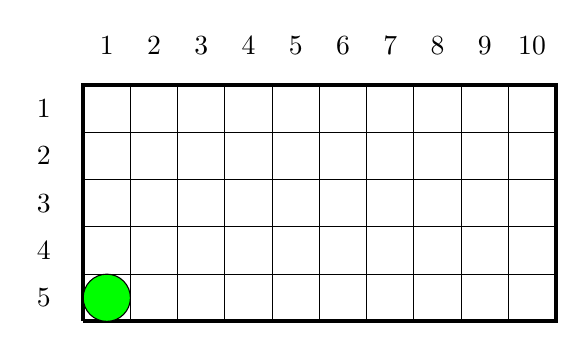
\begin{tikzpicture}
% Drawing environment
\draw[thick, line width=1.5pt] (0,0)--(6,0)--(6,3)--(0,3)--(0,0);

% Draw Robot
\draw[fill=green] (0.3,0.3) circle (0.3);

% Draw vertical lines
\draw (0.6,0) -- (0.6,3);
\draw (1.2,0) -- (1.2,3);
\draw (1.8,0) -- (1.8,3);
\draw (2.4,0) -- (2.4,3);
\draw (3,0) -- (3,3);
\draw (3.6,0) -- (3.6,3);
\draw (4.2,0) -- (4.2,3);
\draw (4.8,0) -- (4.8,3);
\draw (5.4,0) -- (5.4,3);
\draw (6,0) -- (6,3);

% Draw horizontal lines
\draw (0,0.6) -- (6,0.6);
\draw (0,1.2) -- (6,1.2);
\draw (0,1.8) -- (6,1.8);
\draw (0,2.4) -- (6,2.4);
\draw (0,3) -- (6,3);

% Label hz nodes
\node (1h) at (0.3,3.5) {1};
\node (2h) at (0.9,3.5) {2};
\node (3h) at (1.5,3.5) {3};
\node (4h) at (2.1,3.5) {4};
\node (5h) at (2.7,3.5) {5};
\node (6h) at (3.3,3.5) {6};
\node (7h) at (3.9,3.5) {7};
\node (8h) at (4.5,3.5) {8};
\node (9h) at (5.1,3.5) {9};
\node (10h) at (5.7,3.5) {10};

% Label vert nodes
\node (1v) at (-0.5,2.7) {1};
\node (2v) at (-0.5,2.1) {2};
\node (3v) at (-0.5,1.5) {3};
\node (4v) at (-0.5,0.9) {4};
\node (5v) at (-0.5,0.3) {5};
\end{tikzpicture}
\caption{Since the environment dimensions are known ahead of time, the environment can be discretised into robot sized segments (note that the robot's dimensions are illustrated by the green circle). This allows the robot to exploit this structure to systematically explore the environment for the red exit panel.}
\end{minipage}
\hspace{1cm}
\begin{minipage}[c]{0.45\textwidth}
\centering
\captionof{table}{A 3D array struction is used by creating an array of length 6, which is stored in each grid location}
\small\begin{tabular}{cp{5cm}}
\toprule
\textbf{Array Index} & \textbf{Information Stored}\\
\midrule
 & \\
0 & visited (v) or unknown (u)\\
 & \\
1 & direction that the robot faced the first time it visited the spot (f,b,l,r)\\
 & \\
2,3,4 & left, front, and right sides: wall (w), no wall (o), exit (x)\\
 & \\
5 & the direction from which the robot leaves the location with respect to the direction that the robot faces: forward (3), right (2), left (1)\\
 & \\
\bottomrule
\end{tabular}
\end{minipage}
\end{figure}

This scheme would provide higher levels of assurance that the robot will traverse the full map and arrive at the exit panel, however, this implementation runs the risk of exceeding the 3 minute time limit - it is easy to imagine a scenario in which the exit is located in the final panel visited.

\begin{table}[h]
\centering
\caption{Advantages, disadvantages and the hardware requirements for the moderate complexity design option}
\small\begin{tabular}{p{8cm}p{8cm}}
\toprule
\textbf{Advantages} & \textbf{Disadvantages}\\
\midrule
\begin{itemize}\item Robot will try to traverse the entire map, looking for the exit zone since the robot will systematically move through the environment \item Relatively easy to build the software \item Only requires minor additional hardware compared to low complexity design \end{itemize} &
\begin{itemize}\item Runs the risk of exceeding the maximum time of 3 minutes to find the exit \item Environment topologies may exist that cause the robot to believe areas of the environment are inaccessible \end{itemize}\\
\midrule
\textbf{Hardware Requirements} & \\
\midrule
\begin{itemize}\item Rover 5 chassis \item NI MyRio Xilinx 7Z2010 processor \item 4 Channel motor control unit \end{itemize} & \begin{itemize} \item 3 $\times$ SHARP GP2D120 \item 1 $\times$ SHARP GP2Y0A21YK0F \item 1 $\times$ PING))) Ultrasonic distance sensor \end{itemize}\\
\bottomrule
\end{tabular}
\end{table}

\subsection{High Design Complexity}
The previous two design options are best suited to basic environments, like the one shown in Figure 7. This environment has obstacles with surfaces that are orthogonal or parallel to other obstacle surfaces. The design options shown in Sections 4.1 and 4.2 may start to encounter difficulties when presented environments that are more complex, like that shown in Figure 7.
\begin{figure}[h]
\centering
\begin{minipage}{0.45\textwidth}
\centering
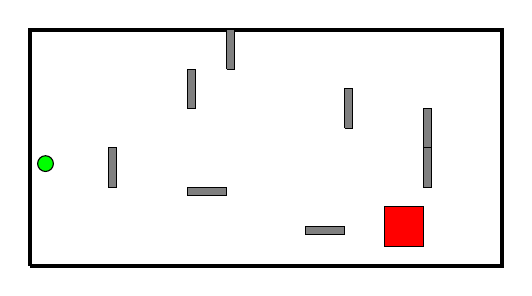
\begin{tikzpicture}
% Drawing environment
\draw[thick, line width=1.5pt] (0,0)--(6,0)--(6,3)--(0,3)--(0,0);
\draw[fill=gray] (1,1) -- (1.1,1) -- (1.1,1.5) -- (1,1.5) --(1,1);
\draw[fill=gray, cm={cos(0) ,-sin(0) ,sin(0) ,cos(0) ,(1,1)}] (1,1) -- (1.1,1) -- (1.1,1.5) -- (1,1.5) --(1,1);
\draw[fill=gray, cm={cos(90) ,-sin(90) ,sin(90) ,cos(90) ,(1,2)}] (1,1) -- (1.1,1) -- (1.1,1.5) -- (1,1.5) --(1,1);
\draw[fill=gray, cm={cos(0) ,-sin(0) ,sin(0) ,cos(0) ,(4,0.5)}] (1,1) -- (1.1,1) -- (1.1,1.5) -- (1,1.5) --(1,1);
\draw[fill=gray, cm={cos(0) ,-sin(0) ,sin(0) ,cos(0) ,(3,0.75)}] (1,1) -- (1.1,1) -- (1.1,1.5) -- (1,1.5) --(1,1);
\draw[fill=gray, cm={cos(0) ,-sin(0) ,sin(0) ,cos(0) ,(1.5,1.5)}] (1,1) -- (1.1,1) -- (1.1,1.5) -- (1,1.5) --(1,1);
\draw[fill=gray, cm={cos(90) ,-sin(90) ,sin(90) ,cos(90) ,(2.5,1.5)}] (1,1) -- (1.1,1) -- (1.1,1.5) -- (1,1.5) --(1,1);
\draw[fill=gray, cm={cos(0) ,-sin(0) ,sin(0) ,cos(0) ,(4,0)}] (1,1) -- (1.1,1) -- (1.1,1.5) -- (1,1.5) --(1,1);

% Drawing exit square
\draw[fill=red, cm={cos(0), -sin(0), sin(0), cos(0), (4.5,0.25)}] (0,0) -- (0.5,0) -- (0.5,0.5) -- (0,0.5) -- (0,0);

% Drawing robot
\draw[fill=green] (0.2,1.3) circle (0.1cm);
\end{tikzpicture}
\caption{An example of a low complexity environment with obstacles having parallel or orthogonal surfaces}
\end{minipage}
\hspace{1cm}
\begin{minipage}{0.45\textwidth}
\centering
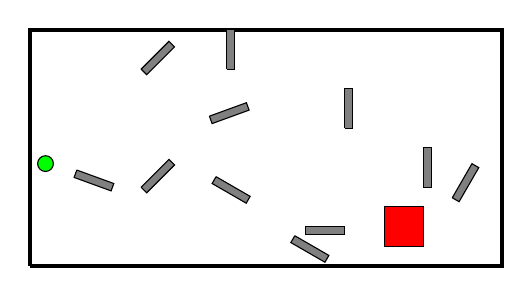
\begin{tikzpicture}
% Drawing environment
\draw[thick, line width=1.5pt] (0,0)--(6,0)--(6,3)--(0,3)--(0,0);

% Drawing obstacle
\draw[fill=gray, cm={cos(45) ,-sin(45) ,sin(45) ,cos(45) ,(0,1)}] (1,1) -- (1.1,1) -- (1.1,1.5) -- (1,1.5) --(1,1);
\draw[fill=gray, cm={cos(30) ,-sin(30) ,sin(30) ,cos(30) ,(4,0.5)}] (1,1) -- (1.1,1) -- (1.1,1.5) -- (1,1.5) --(1,1);
\draw[fill=gray, cm={cos(120) ,-sin(120) ,sin(120) ,cos(120) ,(2,2.5)}] (1,1) -- (1.1,1) -- (1.1,1.5) -- (1,1.5) --(1,1);
\draw[fill=gray, cm={cos(45) ,-sin(45) ,sin(45) ,cos(45) ,(0,2.5)}] (1,1) -- (1.1,1) -- (1.1,1.5) -- (1,1.5) --(1,1);
\draw[fill=gray, cm={cos(120) ,-sin(120) ,sin(120) ,cos(120) ,(3,1.75)}] (1,1) -- (1.1,1) -- (1.1,1.5) -- (1,1.5) --(1,1);
\draw[fill=gray, cm={cos(110) ,-sin(110) ,sin(110) ,cos(110) ,(0,2.5)}] (1,1) -- (1.1,1) -- (1.1,1.5) -- (1,1.5) --(1,1);
\draw[fill=gray, cm={cos(70) ,-sin(70) ,sin(70) ,cos(70) ,(1,2.5)}] (1,1) -- (1.1,1) -- (1.1,1.5) -- (1,1.5) --(1,1);

\draw[fill=gray, cm={cos(0) ,-sin(0) ,sin(0) ,cos(0) ,(3,0.75)}] (1,1) -- (1.1,1) -- (1.1,1.5) -- (1,1.5) --(1,1);
\draw[fill=gray, cm={cos(0) ,-sin(0) ,sin(0) ,cos(0) ,(1.5,1.5)}] (1,1) -- (1.1,1) -- (1.1,1.5) -- (1,1.5) --(1,1);
\draw[fill=gray, cm={cos(90) ,-sin(90) ,sin(90) ,cos(90) ,(2.5,1.5)}] (1,1) -- (1.1,1) -- (1.1,1.5) -- (1,1.5) --(1,1);
\draw[fill=gray, cm={cos(0) ,-sin(0) ,sin(0) ,cos(0) ,(4,0)}] (1,1) -- (1.1,1) -- (1.1,1.5) -- (1,1.5) --(1,1);

% Drawing exit square
\draw[fill=red, cm={cos(0), -sin(0), sin(0), cos(0), (4.5,0.25)}] (0,0) -- (0.5,0) -- (0.5,0.5) -- (0,0.5) -- (0,0);

% Drawing robot
\draw[fill=green] (0.2,1.3) circle (0.1cm);
\end{tikzpicture}
\caption{An example of a more complex environment which has obstacle surfaces at angles, providing more opportunities for simple system failure.}
\end{minipage}
\end{figure}

This is because obstacles may fall across multiple grid regions, or simply because the variability of obstacle angles create more permutations of environments in which a simple robot may get trapped. This would increase the difficulty involved with ensuring that each of these unique 'trapping' environments are considered. A more robust solution for dealing with complex environments, would be to use more sophisticated sensors to map the environment with higher fidelity.

\begin{figure}[h]
\centering
\includegraphics[height=4cm]{image4}
\caption{The picture on the left shows an image captured by an RGB camera mounted to the front of the robot, and the picture on the right shows a transformation of the original image for navigational purposes}
\end{figure}

\begin{figure}[h]
\centering
\includegraphics[height=4cm]{image7}
\caption{Using a simple RGB (or HSV) segmentation filter, the navigable terrain is highlighted to use for obstacle avoidance}
\end{figure}

There are a number of different options when looking at more sophisticated sensors. Some of these include optical (RGB) cameras, optical with IR depth (RGBD) cameras, or Lidar. The later two sensors provide advanced options like developing point clouds of an environment, but are considerably more costly. An example showing a simple RGB camera mounted to the front of the robot can be seen in Figure 8. The image from the robot camera is transformed to aid conceptualisation of the environment map - this step is purely aesthetic. Figure 9 shows the segmentation of navigable terrain and obstacles using a HSV filter. Advanced sensors provide rich environmental information sets, which allow for more sophisticated mapping and navigation algorithms. According to Cadena, et alias (2016), simultaneous localisation and mapping (SLAM) is widely employed in autonomous robotics. SLAM allows simultaneous estimation of robot state ($x$-coord, $y$-coord, $z$-coord, roll, pitch, yaw), and mapping of the environment. Much less sophisticated techniques, such as using odometry for mapping, tend to accumulate error over time. SLAM provides a 'reset' of these errors by revisiting previously mapped areas. This approach allows robust accurate mapping, and efficient location of the exit zone, meaning the robot can reach it's objective faster.

\begin{table}[h]
\centering
\caption{Advantages, disadvantages and the hardware requirements for the design option}
\small\begin{tabular}{p{8cm}p{8cm}}
\toprule
\textbf{Advantages} & \textbf{Disadvantages}\\
\midrule
\begin{itemize}\item Higher fidelity mapping \item Reduced errors in navigation \item Rapid navigation to exit zone\end{itemize} &
\begin{itemize}\item Sensors are costly \item Technically challenging to implement \item Runs the risk of 'over engineering' a solution\end{itemize}\\
\midrule
\textbf{Hardware Requirements} & \\
\midrule
\begin{itemize}\item Rover 5 chassis \item NI MyRio Xilinx 7Z2010 processor \item 4 channel motor controller \end{itemize} & \begin{itemize} \item 3 $\times$ SHARP GP2D120 \item Intel 82634DSB2P RealSense R200 Camera \item (OR) Scanse Lidar Sweep Scanner \end{itemize}\\
\bottomrule
\end{tabular}
\end{table}
%------------------------------------------------------
\section{Project Management}
\subsection{Project Personnel}
This project requires both technical and non-technical skills. The success of the project depends on the efficiency and productivity of the team. The delegation of tasks has been distributed amongst the group based on individual strengths and weaknesses. This will assist the team to work efficiently on each task. The expectation of the team is that each member of the group contributes to the project in accordance with the breakdown Table below.

\begin{table}[h]
\centering
\caption{Project Personnel}
\small\begin{tabular}{lp{5cm}p{5cm}}
\toprule
\textbf{Name} & \textbf{Technical Contribution} & \textbf{Non-Technical Contribution}\\
\midrule
 & & \\
Shane Reynolds & Programming, software integration and hardware assembly, testing, code troubleshooting & Team Leader//Report preparation\\
 & & \\
Tatyana Maltseva & Vehicle assembly, hardware integration, testing, programming assistance & Report writing, research and information gathering, presentation preparation\\
 & & \\
Sakon Nadthayai & Vehicle assembly, hardware integration, testing, programming assistance & Report writing, research and information gathering, presentation preparation\\
& & \\
\bottomrule
\end{tabular}
\end{table}

\subsection{Project Plan}
The complexity of this design project requires a structural logical approach. Hence its imperative to detail a project plan to ensure that the project is completed in a timely manner and to a high standard. A sequence of tasks was created to identify all important due dates. The Figure below shows the main milestones and the duration of each phase. Each phase consists of necessary tasks to complete the design, construction and implementation of the autonomous robotic vehicle. For more information about each phase and its tasks, please refer to Gantt Chart on page 8.\\

\begin{figure}[h]
\centering
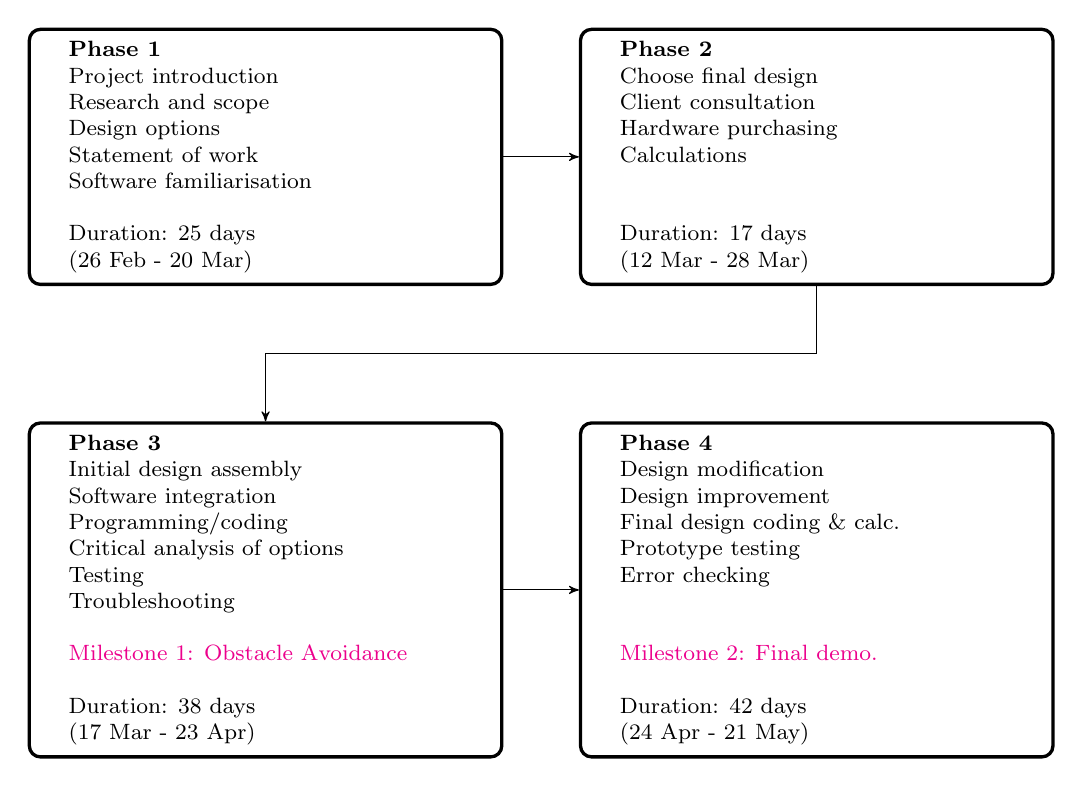
\begin{tikzpicture}[->,>=stealth', node distance=7cm]
\node[rectangle, rounded corners, minimum width=6cm, draw=black, very thick] (phase1)
{\footnotesize\begin{tabular}{p{5cm}}
 \textbf{Phase 1}\\
 Project introduction\\
 Research and scope\\
 Design options\\
 Statement of work\\
 Software familiarisation\\
 \\
 Duration: 25 days\\
 (26 Feb - 20 Mar)
\end{tabular}};

\node[rectangle, rounded corners, minimum width=6cm, draw=black, very thick, right of=phase1] (phase2)
{\footnotesize\begin{tabular}{p{5cm}}
 \textbf{Phase 2}\\
 Choose final design\\
 Client consultation\\
 Hardware purchasing\\
 Calculations\\
 \\
 \\
 Duration: 17 days\\
 (12 Mar - 28 Mar)
\end{tabular}};

\coordinate[below of=phase1, yshift=4.5cm] (stop1) {};
\coordinate[below of=phase2, yshift=4.5cm] (stop2) {};

\node[rectangle, rounded corners, minimum width=6cm, draw=black, very thick, below of=stop1, yshift=4cm] (phase3)
{\footnotesize\begin{tabular}{p{5cm}}
 \textbf{Phase 3}\\
 Initial design assembly\\
 Software integration\\
 Programming/coding\\
 Critical analysis of options\\
 Testing\\
 Troubleshooting\\
 \\
 \textcolor{magenta}{Milestone 1: Obstacle Avoidance}\\
 \\
 Duration: 38 days\\
 (17 Mar - 23 Apr)
\end{tabular}};

\node[rectangle, rounded corners, minimum width=6cm, draw=black, very thick, below of=stop2, yshift=4cm] (phase4)
{\footnotesize\begin{tabular}{p{5cm}}
 \textbf{Phase 4}\\
 Design modification\\
 Design improvement\\
 Final design coding \& calc.\\
 Prototype testing\\
 Error checking\\
 \\
 \\
 \textcolor{magenta}{Milestone 2: Final demo.}\\
 \\
 Duration: 42 days\\
 (24 Apr - 21 May)
\end{tabular}};

\draw[->] (phase1) -- (phase2);
\draw (phase2) -- (stop2) -| (stop1) -- (phase3);
\draw[->] (phase3) -- (phase4);
\end{tikzpicture}
\caption{Phase description of the project, providing an overview of the project timeline, and highlighting key deliverables and milestones}
\end{figure}

From the Figure above it can be seen that the longest phases of the project are 2 and 3. These phases comprise the most challenging elements and two major milestones of the project i.e. completion of the robotic vehicle electrically and mechanically, development of working algorithm, design calculations, testing and troubleshooting and finally completing technical report. 

%------------------------------------------------------
\section{Project Stakeholders}
The identification of the project stakeholders is a primary task of any project. Project stakeholders are those groups/individuals that design and execute the project; change project direction if necessary; and last but not least  decide on the outcome of the project thus it's imperative to acknowledge all the stakeholders of the project.\\

The stakeholders of this project are as follows:
\begin{itemize}
\item \textbf{Client} - Erwin Chan, Rob Wolff, Charlie
\item \textbf{Design team} - Shane Reynolds, Sakon Nadthayai, Tatyana Maltseva  
\end{itemize}

%------------------------------------------------------
\section{Budget Estimates}
Each of the three design options require the use of the Rover 5 chassis, the 4 channel motor controller, and the NI myRio Xilinx processor. The main differentiation in terms of cost comes down to the sensors that will be employed and the estimated man hours involved with the implementation. Table 7 provides the estimated budget for each option.
\begin{table}[h]
\centering
\caption{text}
\begin{tabular}{p{6cm}rp{6cm}r}
\toprule
\textbf{Sunk Costs} & & \textbf{Low Complexity} & \\
\midrule
Rover 5 chassis & \$128.00 & 3 $\times$ SHARP GP2D120 & \$ \\
myRio 1900 & \$814.00 & 1 $\times$ SHARP GP2Y0A21YK0F & \$ \\
4 channel motor controller & \$21.95 &  & \$ \\
\midrule
Total & & Total & \\
\midrule
\midrule
\textbf{Moderate Complexity} & & \textbf{High Complexity} & \\
\midrule
\midrule
Total & & Total & \\
\bottomrule
\end{tabular}
\end{table}

%------------------------------------------------------
\section{Project Constraints}
The project has 3 limitations that can be considered as constraints including;
\begin{itemize}
\item \textbf{Cost}: for achieving of design the robot performing effectively as a client requirement, it requires to use a high quality of camera for example, a RGBD camera and a number of sensors to increase a performance of the robot to move and check obstacles faster and more accurate. Therefore,it can affect an increasing of budgeting.
\item \textbf{Time}: because of a short time period of the completed project which is only 11 weeks the project has to completely finish building a perfect robot that can work perfectly as the client requirement, during a process of designing to implementing the autonomous robotic vehicle , it requires time to test, evaluate, study,search and improve to make the robot working perfectly. Thus, as the limitation of time may affect the quality of the robot performance. Also a delivery time of ordered any material parts might affect the time frame.
\item \textbf{Scope}: as the limitation of the project scope and the client requirement affect cost,time frame and quality in the project, if one factor is changed this will affect to other factor. However, this project is focusing on the quality of the robotic performance  therefore the cost and the time are required more.
Quality; because of the limitation of the budget and the time frame in this project it affects to the quality of the robotic performance. As an extend of the budgeting and time frame will make high quality of the autonomous robotic vehicle performance.
\end{itemize}

%------------------------------------------------------
\section{Preferred Design \& Points for Discussion}
The preferred design option is one which meets the project requirements an operates within the project constraints, whilst delivering an optimal outcome for performance and cost. In reality, the best solution is most likely to include elements from the low, moderate, and high complexity design options - there are useful design elements in each. The most robust solution would be the 
\begin{table}[h]
\centering
\caption{Additional information that needs to be sought for effective selection of robot design}
\begin{tabular}{p{8cm}p{8cm}}
\toprule
\textbf{Environment Questions} & \textbf{Other Questions}\\
\midrule
What materials is the environment constructed with? & Will the location of the exit zone always be in the same sport? Or will the location be random?\\
Does the environment change, or will it be the same topology? & Will the location of the exit have any defining characteristics (e.g. located next to a wall) \\
Is there access to a test environment? & Is the project restricted to using NI myRio hardware?\\
Does the entrance to the environment always start at the same point, or is it randomised? & \\
Will the walls and obstacles be assigned with parallel, and orthogonal surfaces? & \\
Will the environment be based on a grid? Or will the environment be random? & \\
\bottomrule
\end{tabular}
\end{table}

%------------------------------------------------------
\section{References}
Cadena, C., Carlone, L., Carrillo, H., Latif, Y., Scaramuzza, D., Neira, J., Reid, I., \& Leonard, J. (2016). Past, Present, and Future of Simultaneous Localisation and Mapping: Towards the Robust-Perception Age. \textit{IEEE Transactions on Robotics}, 32 (6) pp 1309-1332\\

Kapoor, S., Mahesh, K., Ruzinov, D., Battipaglia, J. (2017). Autonomously Solving Mazes with Robots. Retrieved from \small\url{http://soe.rutgers.edu/sites/default/files/imce/gov2017/Autonomously%20Solving%20Mazes%20with%20Robots.pdf}\\

Kumar, R., Jitoko, P., Kumar, S., Pillay, K., Prakash, P., Sagar, A.,...Mehta, U. (2016). Maze solving robot with automated obstacle avoidance. Paper presented at: \textit{2016 IEEE International Symposium on Robotics and Intelligent Sensors, Tokyo, Japan.}\\



%------------------------------------------------------

\begin{sidewaysfigure}[p]
\centering
\includegraphics[scale=0.38]{gantt}
\caption{text}
\end{sidewaysfigure}

\end{document}